\documentclass[conference]{IEEEtran}
\usepackage{cite}
\usepackage{amsmath,amssymb,amsfonts}
\usepackage{algorithmic}
\usepackage{graphicx}
\usepackage{textcomp}
\usepackage{xcolor}
\usepackage{hyperref}
\usepackage{caption}

\captionsetup{font=normal}

\newcommand{\note}[1]{\textsf{\color{red}{[{NOTE: #1}]}}}
\newcommand{\jin}[1]{\textsf{\color{purple}{[{Jin: #1}]}}}
\newcommand{\larry}[1]{\textsf{\color{purple}{[{Larry: #1}]}}}
\newcommand{\kaiqi}[1]{\textsf{\color{blue}{[{Kaiqi: #1}]}}}
\newcommand{\michael}[1]{\textsf{\color{blue}{[{Michael: #1}]}}}
\newcommand{\woojin}[1]{\textsf{\color{blue}{[{Woojin: #1}]}}}
\newcommand{\corey}[1]{\textsf{\color{blue}{[{Corey: #1}]}}}


\def\BibTeX{{\rm B\kern-.05em{\sc i\kern-.025em b}\kern-.08em
    T\kern-.1667em\lower.7ex\hbox{E}\kern-.125emX}}
    
\begin{document}

\title{Secure Coding with LLMs - Title TBD\\

\thanks{Identify applicable funding agency here. If none, delete this.}
}

\author{
\IEEEauthorblockN{1\textsuperscript{st} Kaiqi Liang}
\IEEEauthorblockA{\textit{CSSE Department} \\
\textit{University of Western Australia}\\
Perth, WA \\
23344153@student.uwa.edu.au}
\and
\IEEEauthorblockN{2\textsuperscript{nd} Corey Saxon}
\IEEEauthorblockA{\textit{CSSE Department} \\
\textit{University of Western Australia}\\
Perth, WA \\
23178835@student.uwa.edu.au}
\and
\IEEEauthorblockN{3\textsuperscript{rd} Michael Hodgson}
\IEEEauthorblockA{\textit{CSSE Department} \\
\textit{University of Western Australia}\\
Perth, WA \\
email address or ORCID}
\and
\IEEEauthorblockN{4\textsuperscript{th} Woojin Jeon}
\IEEEauthorblockA{\textit{Dept. of Electrical and Computer Engineering} \\
\textit{Sungkyunkwan University}\\
Suwon, Korea \\
dnwls0116@naver.com}
\and
\IEEEauthorblockN{5\textsuperscript{th} Larry Huynh}
\IEEEauthorblockA{\textit{dept. name of organization (of Aff.)} \\
\textit{name of organization (of Aff.)}\\
City, Country \\
email address or ORCID}
\and
\IEEEauthorblockN{6\textsuperscript{th} Jin Hong}
\IEEEauthorblockA{\textit{dept. name of organization (of Aff.)} \\
\textit{name of organization (of Aff.)}\\
City, Country \\
email address or ORCID}
}

\maketitle

\begin{abstract}
Despite its widespread use in industry and academia, the security of code generated by large language models (LLMs) has not had much research done towards it. Our group aims to fill this knowledge gap through the application of static analysis tools and integration with the GPT4 API. By performing an iterative process of analysis and improvement, our pipeline can identify vulnerabilities in provided code and suggest prompts which may assist a user in constructing a prompt to initiate a response of secure code from GPT. Prompt engineering techniques are leveraged to best instruct the model how to perform these tasks and act in a predictable manner.

\corey {DO THE ABSTRACT LAST}
\end{abstract}

\begin{IEEEkeywords}
prompt engineering, static analysis, large-language model, secure code generation
\end{IEEEkeywords}

\section{Introduction}
LLMs have been making waves in many fields since their introduction. Their prevalence and ubiquity are undeniable, but their use is considered hazardous \corey{DEFINITELY reword this. My brain is failing me} due to their own non-deterministic nature \corey{I think we have a source to support this, if not I'll find one.}.
Due to their popularity and inherent danger, the accuracy of their output has need to be assessed. Focusing on the field of secure coding, our aim is to investigate how often GPT provides codes with security vulnerabilities and how different kinds of prompting techniques change the presence of such vulnerabilities. 
This is done with the desirable outcome of providing a tool which not only improves the security of code output by GPT, but also assist the user in their prompt-writing to assure that future queries are more likely to result in secure code.

\larry{state the problem and briefly describe how we propse to fix. this is where you inteoduxe the context. something  like with LLMs, it may be possible to produce secure code; we want to investigate how. we provide pupepline for secure code generatoon with ... then give breif statement about outcome of the project}


\section{Related Works}

Due to the fast-paced evolution of OpenAI and it's products, there are little to no papers exploring the newer models of GPT and its application to secure coding. There are some which experiment with GPT3 and GPT3.5, and these are considered relevant enough to be used as primary sources.

There exists some research which explore the likelihood of vulnerability introduction in GPT-generated code\cite{sandoval2023lost}, however these are often based on highly specialised pieces of code, with little programmatic scope and typically based in a single language. For the few which do consider greater variety in code and language, they do not consider how prompts can be engineered to improve code quality and also do not consider how GPT can be used to iteratively improve the code\cite{khoury2023secure}. Other research looks into the generation of code resistant to hardware vulnerabilities\cite{cryptoeprint:2023/212}\cite{saha2023llm}. This is adjacent to the domain of our research but we focus on software vulnerabilities such as the CWE Top 25.
A futher aspect of our research is concerned with prompt engineering and best practices. Researchers have worked on training a model to generate code and experimented with prompt design for that regard, but do not focus on code security in a meaningful way and neglect to consider the ease of model oversight\cite{liu2023improving}\cite{siddiq2023lightweight}.
More common is research concerned with the application of GPT as a bug-fixing tool. It is typically agreed upon that ChatGPT is capable of outperforming traditional bug-fixing tools\cite{sobania2023analysis}\cite{chen2021evaluating}\cite{QuixbugsOpenAIEvaluation}. These papers fail to consider the generation of code by an LLM, and also rely on some manner of manual code review within their system. We hope to avoid this mandatory human involvement as much as possible by introducing GPT as a generator and static analysis tool, performing an iterative improvement 

\larry{try to make more generalized statements about what people did, rather than assessing each one individually. so something like "few previous works have attempted to generate/assess secure code via llms cite(1,2,3). while they have seen success, these works fail to consider (x, y, z), or don't fulfil some standard/requirement. In addition, these works provide single-shot, standalone assessments of security vulnerabilities; we believe these ideas can be enhanced through an iterative improvement model (briefly describe). We are aware of such methods being used in general/in other areas (cite works that have done similar), however (whatever sets us apart, maybe talk about static analysis tools, etc.)}

This is where we aim to abridge previous works by considering generated code and then applying some of these earlier attempted practices.

\section{Pipeline}
\ref{fig:Pipeline}
\begin{figure}[!h]
    \centering
    %\hspace*{-0.3in}
    \centerline{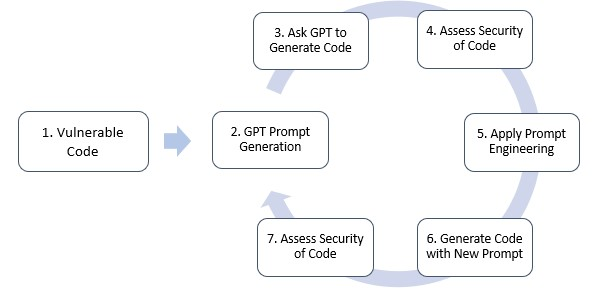
\includegraphics[width=0.5\textwidth]{figures/Pipeline.jpg}}
    \caption{The major steps of the system pipeline}
    \label{fig:Pipeline}
\end{figure}

\begin{figure}
    \centering
    \centerline{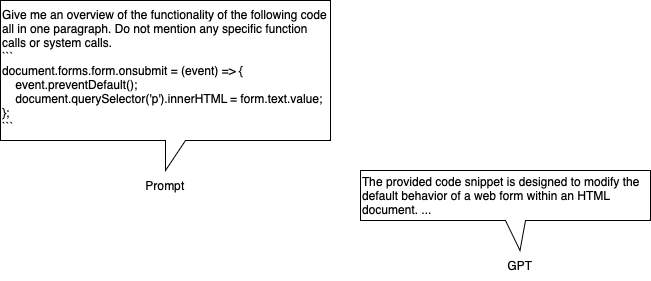
\includegraphics[width=0.5\textwidth]{figures/description_prompt.png}}
    \caption{Prompt for Step 2 of the Pipeline}
    \label{fig:description_prompt}
\end{figure}

\begin{figure}
    \centering
    \centerline{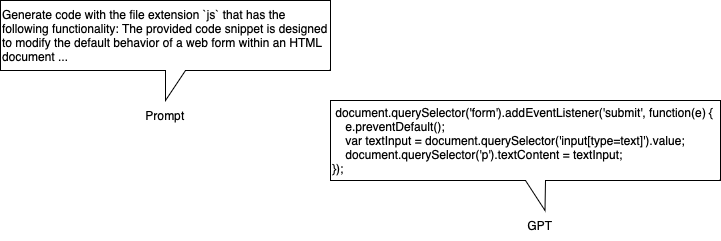
\includegraphics[width=0.5\textwidth]{figures/code_prompt.png}}
    \caption{Prompt for Step 3 of the Pipeline}
    \label{fig:code_prompt}
\end{figure}

\begin{figure*}[!h]
    \centering
    %\hspace*{-0.3in}
    \centerline{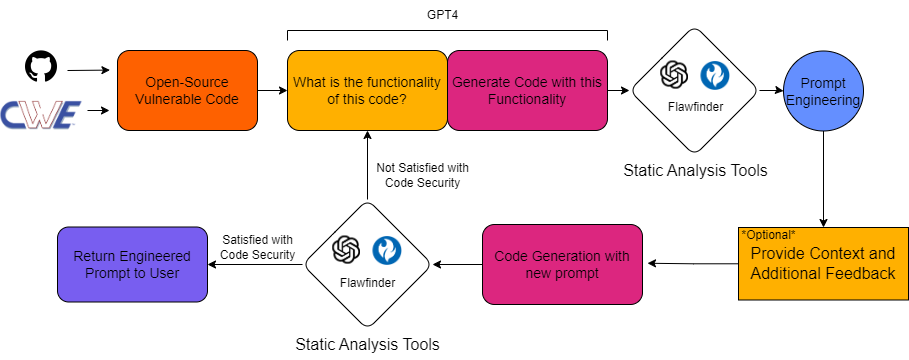
\includegraphics[width=0.9\textwidth]{figures/flowchart.drawio.png}}
    \caption{How some vulnerable code may be processed by the pipeline}
    \label{fig:Flowchart}
\end{figure*}

\larry{add figure for actual pipeline implementation. think design drawings and flowcharts}

\subsection{Step 1: Vulnerable Code}
Vulnerable code snippets, which are fed to the LLM, are sourced from the \href{https://cwe.mitre.org/top25/archive/2023/2023_top25_list.html}{2023 CWE Top 25 Most Dangerous Software Weaknesses}. Most weaknesses include vulnerable code snippets for several languages under the Demonstrative Examples section.
\larry{change the remaining part to just something like "we also account for variety of most popular programming languages. then also make the observation that certain vulnerabilities and analysis tools are language specific, and give examples. then just say our model is robust to this.}
Different languages were considered for their unique vulnerabilities but also to assess the scope of application of this pipeline. Currently, code built in C/C++, Python, Java, JavaScript and TypeScript are run over chosen static analyzers, where other languages will skip the step of static analysis.

\subsection{Step 2: GPT Prompt Generation}
In this step we ask GPT to generate a prompt given the vulnerable code which can be used in the next step to generate code. Given the vulnerable code, we initially form a prompt that requests GPT to write another prompt, which once given back to GPT should generate a version of the original code with the vulnerability removed. Shown in Figure \ref{fig:description_prompt} is an example of a prompt used for the XSS vulnerability.

\subsection{Step 3: Code Generation}
Next we used the prompt generated in the previous step and asked GPT to give us code described by the prompt. An example is shown in Figure \ref{fig:code_prompt}.

\verb|extension| makes sure that the code GPT generates next is in the same programming langauge as the vulnerable code.
\subsection{Step 4: Security Assessment}
Here is where our static analysis tools come in. Once the testable code has been generated, it must be assessed by some metric to measure how vulnerable it is. Several tools were considered but most were ultimately deemed unusable in our pipeline. This was due to either their inability to identify simple vulnerabilities shown to them or their lack of command line control options. If these tools worked solely as IDE plug-ins, they would not be suitable for an automated pipeline.
These tools must also possess several properies which would make their use suitable. Their result format must be mostly \textit{deterministic}, so that results are reproducible and to prevent divergent loops where a previously identified vulnerability is no longer found, despite it not being fixed. The tools must also have an expected output so that they may be parseable by the pipeline, and must have an acceptable degree of abstraction so that while training and developing the system we can identify any potential shortcomings.

\corey{Considering adding a table depicting tools considered and why they were/werent accepted (tool, ability to find simple vuln, terminal control, accepted)}

\subsubsection{SonarQube}
While SonarQube is a widely used open- source platform for analyzing and tracking the quality of code \cite{8813272} but it is a very complex software with a user interface which is difficult to integrate with a command line tool. Hence we opt out of that.
\subsubsection{HCL AppScan}
Great as an IDE plugin but hard to build into a pipeline run on the command line.
\subsubsection{Flawfinder}
Easy to set up, sometimes perform as well as the other open source tools\cite{bitdefendercomparison}.
\subsubsection{SpotBugs}
Better than PMD for Java \cite{KAUR20202023}.
\subsubsection{Bearer CLI}
Static Application Security Testing (SAST) to discover, filter and prioritize security and privacy risks using sensitive data flow analysis. Currently supports Java, Ruby, JavaScript and TypeScript.
\subsubsection{Bandit}
Bandit is a comprehensive source vulnerability scanner for Python.

\subsection{Step 5: Prompt Engineering}
Prompt engineering is the refinement of the prompts fed to LLMs to direct and manipulate the model to create predictable output. 
There are several techniques which assisted in our prompt engineering practices: 
\begin{enumerate}
    \item Clarity and Specificity
    \item Context and Background Information
    \item Tone and Style
    \item Brevity and Focus
    \item Goal Orientation
    \cite{promptengineeringbestpractices}
\end{enumerate} 
An effective prompt should convey exactly what is expected to the LLM to provide relevant output. Contextual cues aid the model in understanding the role the code will play in the system and thus adjust its responses accordingly. The tone of the prompt used can influence the manner in which the model gives it outputs. While providing context is important, overly long prompts can confuse the model and dilute the users original intent. It is also important to have a clear goal in the prompt for the model to properly respond to.

\subsection{Step 6: Generation with new Prompt}
Using this engineered prompt, we generate new code which should now be free of some or all of the identified vulnerabilities.

\subsection{Step 7: Reassessment}
The earlier static analysis techniques are repeated to gauge if the number and severity of vulnerabilities have been reduced. If they have not, the pipeline will iterate again. If the model is satisfied with the improvement of the code, it will return the code along with the prompt that generated that code.

\section{Case Study}
\subsection{Static Analysis Tools}
The traditional static analysis tools had a high rate of false negatives, they were not able to pick up several of the simple example vulnerabilities. The conducted experiments are shown in Table \ref{table:static_analysis_tools}. These results were particularly troubling due to the importance of being able to accurately identify where vulnerabilities exist in code in order to fix them.
\subsection{Static Analysis Using GPT}
Due to static analysis tools' insufficiency for finding vulnerabilities the decision was made to experiment with using GPT4. It was able to identify every single example vulnerability that we tested under the \href{https://cwe.mitre.org/top25/archive/2023/2023_top25_list.html}{2023 CWE Top 25 Most Dangerous Software Weaknesses}. Upon further literature review and with papers supporting GPT's ability as an analysis tool \cite{sobania2023analysis}\cite{QuixbugsOpenAIEvaluation}, GPT was introduced to the pipeline with the additional role as a static analysis tool.
\subsection{Difficult Vulnerability}
\begin{figure}
    \centering
    \centerline{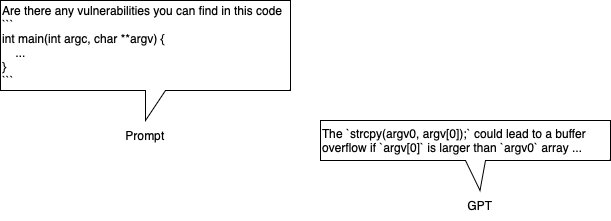
\includegraphics[width=0.5\textwidth]{figures/dnstracer_prompt.png}}
    \caption{Prompt for static analysing dnstracer.c}
    \label{fig:dnstracer_prompt}
\end{figure}
In the two case studies above the vulnerabilities we tested are very stripped down versions whose complexity is not likely to be representative of any real world software. We attempted to see if GPT can identify \href{https://www.cve.org/CVERecord?id=CVE-2017-9430}{CVE-2017-9430}, passing the entire dnstracer.c file to GPT4 exceeded the maximum number of tokens the current state of the model can handle. However we opted to give GPT only the main function and it found the intended Buffer Overflow vulnerability as shown in Figure \ref{fig:dnstracer_prompt}.

\subsection{Iteration}
\corey{We need to properly define what metric we are using to limit our iteration. Is it going until there are no more vulnerabilities, but also with a cap? Is it doing a percentage reduction?}

\section{Testing}
\corey{We should do testing of GPT as a static analysis tool, feeding it vulnerable code and measuring how often it finds the vulnerabilities. This will give us a useful figure but also provide some much-needed authenticity.}

\section{Code Improvement}
\corey{How often is the code improved? By how much? After how many iterations? Should consider building a table depicting languages used, CWEs used, and the actual improvement.}


\begin{table}[!ht]
    \centering
    \caption{List of CWE Vulnerabilities and the Detection Results Using Static Analysis Tools}
    \begin{tabular}{|p{1.8cm}|l|p{1.2cm}|p{1.4cm}|l|}
    % \begin{tabular}{|l|l|l|l|l|l|l|}
        \hline
        \textbf{CWE Vulnerability} & \textbf{CWE ID} & \textbf{Language} & \textbf{Static Analysis Tool} & \textbf{Detected} \\
        \hline
        Out-of-bounds Write & CWE-787 & C & Flawfinder & No \\
        \hline
        XSS & CWE-79 & HTML & HCL AppScan & Yes \\
        \hline
        SQLi & CWE-89 & JavaScript & Bearer & No \\
        \hline
        Use After Free & CWE-416 & C & Flawfinder & No \\
        \hline
        OS Command Injection & CWE-78 & C & Flawfinder & Yes \\
        \hline
        Improper Input Validation & CWE-20 & C & Flawfinder & No \\
        \hline
        Out-of-bounds Read & CWE-125 & Python & Bandit & No \\
        \hline
    \end{tabular}
\label{table:static_analysis_tools}
\end{table}

\section{Conclusion}

\bibliographystyle{IEEEtran}
\bibliography{main.bib}

\end{document}
